% This contents of this file will be inserted into the _Solutions version of the
% output tex document.  Here's an example:

% If assignment with subquestion (1.a) requires a written response, you will
% find the following flag within this document: <SCPD_SUBMISSION_TAG>_1a
% In this example, you would insert the LaTeX for your solution to (1.a) between
% the <SCPD_SUBMISSION_TAG>_1a flags.  If you also constrain your answer between the
% START_CODE_HERE and END_CODE_HERE flags, your LaTeX will be styled as a
% solution within the final document.

% Please do not use the '<SCPD_SUBMISSION_TAG>' character anywhere within your code.  As expected,
% that will confuse the regular expressions we use to identify your solution.

\def\assignmentnum{5 }
% \def\assignmentname{Sentiment Analysis}
\def\assignmenttitle{XCS234 Assignment \assignmentnum}
\input{macros}
\begin{document}
\pagestyle{myheadings} \markboth{}{\assignmenttitle}

% <SCPD_SUBMISSION_TAG>_entire_submission

This handout includes space for every question that requires a written response.
Please feel free to use it to handwrite your solutions (legibly, please).  If
you choose to typeset your solutions, the |README.md| for this assignment includes
instructions to regenerate this handout with your typeset \LaTeX{} solutions.
\ruleskip

\LARGE
2.ci
\normalsize

% <SCPD_SUBMISSION_TAG>_2ci
\begin{answer}
  % ### START CODE HERE ###
  Mean: 0.568, Std: 0.063
  % ### END CODE HERE ###
\end{answer}
% <SCPD_SUBMISSION_TAG>_2ci
\clearpage

\LARGE
2.cii
\normalsize

% <SCPD_SUBMISSION_TAG>_2cii
\begin{answer}
  % ### START CODE HERE ###
  \begin{table}[h!]
  \centering
  \caption{LinUCB with "Popular" Arm Updates}
  \begin{tabular}{|l|c|c|}
  \hline
  \textbf{K Value} & \textbf{Mean} & \textbf{Std} \\ \hline
  500              & 0.441         & 0.082        \\ \hline
  1000             & 0.490         & 0.080        \\ \hline
  2500             & 0.535         & 0.073        \\ \hline
  5000             & 0.556         & 0.066        \\ \hline
  \end{tabular}
  \end{table}

  The "Popular" strategy seems worse than the baseline. I think it's because
  this strategy just reinforce the existing model trend without considering
  the actual user preference.
  % ### END CODE HERE ###
\end{answer}
% <SCPD_SUBMISSION_TAG>_2cii
\clearpage


\LARGE
2.ciii
\normalsize

% <SCPD_SUBMISSION_TAG>_2ciii
\begin{answer}
  % ### START CODE HERE ###
  \begin{table}[h!]
  \centering
  \caption{LinUCB with "Corrective" Arm Updates}
  \begin{tabular}{|l|c|c|}
  \hline
  \textbf{K Value} & \textbf{Mean} & \textbf{Std} \\ \hline
  500              & 0.441         & 0.082        \\ \hline
  1000             & 0.490         & 0.080        \\ \hline
  2500             & 0.535         & 0.073        \\ \hline
  5000             & 0.556         & 0.066        \\ \hline
  \end{tabular}
  \end{table}

  It's interesting that "Corrective" has identical results as "Popular".
  My guess is that the most popular arms may also be the most incorrectly
  predicted arms. This will results in the same effect as Popular strategy,
  where the model will reinforce the existing trend and thus converge to
  the same result.
  % ### END CODE HERE ###
\end{answer}
% <SCPD_SUBMISSION_TAG>_2ciii
\clearpage

\LARGE
2.civ
\normalsize

% <SCPD_SUBMISSION_TAG>_2civ
\begin{answer}
  % ### START CODE HERE ###
  \begin{table}[h!]
  \centering
  \caption{Comparison of Mean Total Fraction Correct Across Strategies}
  \begin{tabular}{|l|c|c|c|c|}
  \hline
  \textbf{K Value} & \textbf{None} & \textbf{Popular} & \textbf{Corrective} & \textbf{Counterfactual} \\ \hline
  500              & 0.568         & 0.441            & 0.441               & \textbf{0.705}          \\ \hline
  1000             & 0.568         & 0.490            & 0.490               & \textbf{0.670}          \\ \hline
  2500             & 0.568         & 0.535            & 0.535               & \textbf{0.618}          \\ \hline
  5000             & 0.568         & 0.556            & 0.556               & \textbf{0.570}          \\ \hline
  \end{tabular}
  \end{table}

  The counterfactual strategy is clearly the best of the three arm update
  strategies. It is the only strategy that consistently performs better
  than the baseline case where no new arms are added.

  I think it's because counterfactual is the only strategy that considers
  all user's preferences.
  % ### END CODE HERE ###
\end{answer}
% <SCPD_SUBMISSION_TAG>_2civ
\clearpage

\LARGE
2.cv
\normalsize

% <SCPD_SUBMISSION_TAG>_2cv
\begin{answer}
  % ### START CODE HERE ###
  \begin{figure}[H]
  \centering
    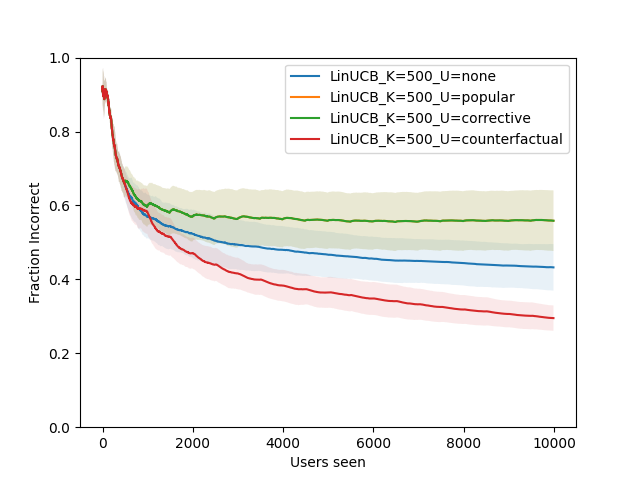
\includegraphics[width=.5\linewidth]{images/fraction_incorrect_2_submission.png}
  \end{figure}
  The counterfactual strategy shows the fastest learning curve and
  the corrective and popular strategies perform worse than the none
  baseline.
  % ### END CODE HERE ###
\end{answer}
% <SCPD_SUBMISSION_TAG>_2cv
\clearpage

\LARGE
2.cvi
\normalsize

% <SCPD_SUBMISSION_TAG>_2cvi
\begin{answer}
  % ### START CODE HERE ###
  \begin{figure}[H]
  \centering
    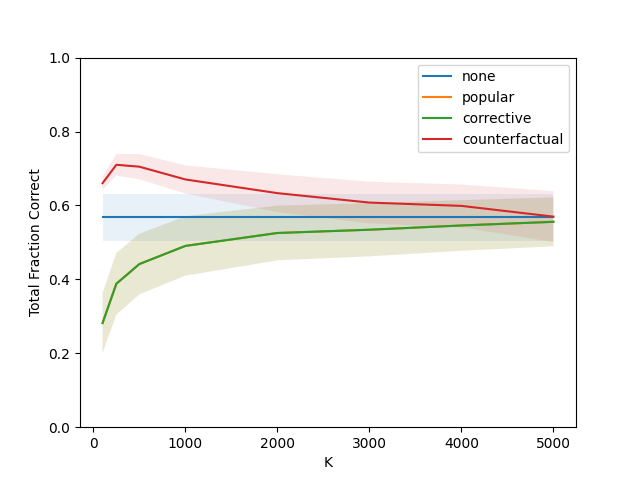
\includegraphics[width=.5\linewidth]{images/k_analysis_submission.png}
  \end{figure}
  \textbf{Getting worse:} The counterfactual perform worse when K is
  getting large. I think this is because smaller values of K allow
  for more frequent adjustments based on recent user interactions.
  \textbf{Getting better:} The popular and corrective strategies
  improve as K increases. I think it's because larger K provides
  a more stable and less noisy signal of what is truly "popular"
  or where "corrective" action is most needed.
  % ### END CODE HERE ###
\end{answer}
% <SCPD_SUBMISSION_TAG>_2cvi
\clearpage



\LARGE
2.d
\normalsize

% <SCPD_SUBMISSION_TAG>_2d
\begin{answer}
  % ### START CODE HERE ###
  \textbf{Ethical issue:} For scenario (1), whether this has ethical
  problem is highly depending on what the user preferences are. In
  scenario (1), eventually, there will be more and more creators
  that only creates contents that meets most of the user preferences.
  The diversity of the content will be very low. If this major trend
  is harmful, then it's a big problem.

  Scenario (2) has a similar issue but worse. It's because the algorithm
  will shift the user preferences to the popular ones and making niche
  contents has less and less opportunities to be seen.

  Scenario (3) is even worse. Instead of randomly selecting contents
  as scenario (2) doing, the popular contents might be manipulated.

  Scenario (4) kind of mitigate the problem where users can intervening
  the algorithm.

  Distinguishing between these scenarios would require specific
  experiments beyond analyzing standard logs.
  % ### END CODE HERE ###
\end{answer}
% <SCPD_SUBMISSION_TAG>_2d
\clearpage

\LARGE
2.e
\normalsize

% <SCPD_SUBMISSION_TAG>_2e
\begin{answer}
  % ### START CODE HERE ###
  I think the platform is primarily responsible for identifying and
  mitigating negative feedback loops because they have direct control
  to the feed algorithms and they has more context to identify possible
  issues. However, all the roles in this loop should be able to recognize
  and have some ways to report the issues to the platform.
  % ### END CODE HERE ###
\end{answer}
% <SCPD_SUBMISSION_TAG>_2e
\clearpage

% <SCPD_SUBMISSION_TAG>_entire_submission

\end{document}
